
\lecture{Measures Of Position}{measures-of-position}
\section{Measures Of Position}


\title{More Measures Of Dispersion}
\subtitle{How Spread Out?}

%\author{Kelly Black}
%\institute{Clarkson University}
\date{20 February 2013}

\begin{frame}
  \titlepage
\end{frame}

\begin{frame}
  \frametitle{Outline}
  \tableofcontents[pausesection,hideothersubsections,sectionstyle=show/hide]
\end{frame}


\iftoggle{clicker}{%
  \subsection{Clicker Quiz}


  \begin{frame}
    \frametitle{Clicker Quiz}

    \vfill
    Find the median of the following data set:\\
    \begin{tabular}{llllll}
      28, & 17, & 12, & 20, & 21, & 18
    \end{tabular}

    \vfill
    
    \begin{tabular}{l@{\hspace{3em}}l@{\hspace{3em}}ll@{\hspace{3em}}l}
      A: 17 & B: 18 & C: 19 & D: 20
    \end{tabular}

    \vfill

  \end{frame}

}




\subsection{Percentiles}

\begin{frame}
  \frametitle{Percentiles}

  \begin{definition}
    The P\textsuperscript{th} percentile is the data point for which P\%
    of the numbers are smaller than it.
  \end{definition}

\end{frame}

\begin{frame}
  \frametitle{Percentiles}

%  \begin{eqnarray*}
%    \begin{array}{lllll}
%      x_1 & x_2 & x_3 & \cdots & x_n \\
%    \end{array}
%  \end{eqnarray*}

  \newcount\xnum
  \newcount\xnumpos
  \only<1>
  {
    \begin{picture}(500,100)(0,0)
      \multiput(10,90)(20, 0){15}{\line(1,0){15}}
      \xnum=1
      \xnumpos=12
      \loop
      \put(\xnumpos,95){$x_{{\the\xnum}}$}
      \advance\xnumpos by 20
      \ifnum\xnum < 15 \advance\xnum by 1
      \repeat
    \end{picture}
  }

  \only<2>
  {
    \begin{picture}(310,100)(0,0)
      \multiput(10,90)(20, 0){15}{\line(1,0){15}}
      \xnum=1
      \xnumpos=12
      \loop
      \put(\xnumpos,95){$x_{{\the\xnum}}$}
      \advance\xnumpos by 20
      \ifnum\xnum < 15 \advance\xnum by 1
      \repeat
      \put(10,0){\line(0,1){80}}
      \put(310,0){\line(0,1){80}}
      \put(110,20){\vector(-1,0){100}}
      \put(210,20){\vector( 1,0){100}}
      \put(120,15){Width=n Items}
    \end{picture}
  }

  \only<3>
  {
    \begin{picture}(310,100)(0,0)
      \multiput(10,90)(20, 0){15}{\line(1,0){15}}
      \xnum=1
      \xnumpos=12
      \loop
      \put(\xnumpos,95){$x_{{\the\xnum}}$}
      \advance\xnumpos by 20
      \ifnum\xnum < 15 \advance\xnum by 1
      \repeat
      \put(10,0){\line(0,1){80}}
      \put(310,0){\line(0,1){80}}
      \put(110,20){\vector(-1,0){100}}
      \put(210,20){\vector( 1,0){100}}
      \put(120,15){Width=n Items}

      \put(250,50){\line(0,1){40}}
      \put(80,60){\vector(-1,0){70}}
      \put(180,60){\vector( 1,0){70}}
      \put(85,55){P Percent of Width}

    \end{picture}
  }

  \vfill
  
\end{frame}

\begin{frame}
  \frametitle{Percentiles}

    \begin{picture}(310,100)(0,0)
      \multiput(10,90)(20, 0){15}{\line(1,0){15}}
      \xnum=1
      \xnumpos=12
      \loop
      \put(\xnumpos,95){$x_{{\the\xnum}}$}
      \advance\xnumpos by 20
      \ifnum\xnum < 15 \advance\xnum by 1
      \repeat
      \put(10,0){\line(0,1){80}}
      \put(310,0){\line(0,1){80}}
      \put(110,20){\vector(-1,0){100}}
      \put(210,20){\vector( 1,0){100}}
      \put(120,15){Width=n Items}

      \put(250,50){\line(0,1){40}}
      \put(70,60){\vector(-1,0){60}}
      \put(190,60){\vector( 1,0){60}}
      \put(75,55){j/n items = k\textsuperscript{th} percent}

    \end{picture}


    \begin{eqnarray*}
      P & = & \frac{k}{100}, \\
      \frac{j}{n} & = & \frac{k}{100}, \\
      \Rightarrow j & = & \frac{nk}{100}.
    \end{eqnarray*}

\end{frame}

\begin{frame}
  \frametitle{Example}

  \vfill 

  Find the 85\textsuperscript{th} percentile for the following data:

  \vfill

  \only<1>
  {
    89, 85, 97 106, 94, 100, 92, 120, 92, 97, 89, 90, 103, 86, 106, 112, 100, 92, 84,
    97, 103, 91, 104, 91, 104
  }

  \only<2>
  {
    Sort it: \\
    84, 85, 86, 89, 89, 90, 91, 91, 92, 92, 92, 94, 97, 97, 97, 100,
    100, 103, 103, 104, 104, 106, 106, 112, 120
  }

  \only<3>
  {
    Sort it: \\
    84, 85, 86, 89, 89, 90, 91, 91, 92, 92, 92, 94, 97, 97, 97, 100,
    100, 103, 103, 104, \underline{104}, \underline{106}, 106, 112, 120
  }


  \vfill

  (There are 25 data points.)

  \vfill

\end{frame}

\begin{frame}
  \frametitle{Clicker Quiz}

  \vfill

  Find the 30\textsuperscript{th} percentile for the following data:

  185, 196, 214, 199, 199, 204


  \vfill

  \begin{tabular}{l@{\hspace{3em}}l@{\hspace{3em}}l@{\hspace{3em}}l}
    A: 185 & B: 193.8 & C: 195 & D: 196
  \end{tabular}



\end{frame}

\subsection{Box Plots}

\begin{frame}{Quartiles}

The 25\textsuperscript{th} and 75\textsuperscript{th} percentiles are
special cases called the first quartile and third quartile
respectively, \\
\begin{tabular}{ll}
  P\textsuperscript{25}: & First Quartile \\
  P\textsuperscript{75}: & Third Quartile \\
\end{tabular}
  
\end{frame}


\begin{frame}{Calculating Quartiles}

  To calculate the quartiles you can use a short cut. Divide the data
  into smaller half and larger half. Then find the medians of the two
  different data sets.

  \vfill

  \only<1>%
  {
    \begin{picture}(310,100)(0,0)
      \multiput(10,90)(20, 0){15}{\line(1,0){15}}
      \xnum=1
      \xnumpos=12
      \loop
      \put(\xnumpos,95){$x_{{\the\xnum}}$}
      \advance\xnumpos by 20
      \ifnum\xnum < 15 \advance\xnum by 1
      \repeat

      \put(10,0){\line(0,1){80}}
      \put(310,0){\line(0,1){80}}
      \put(110,20){\vector(-1,0){100}}
      \put(210,20){\vector( 1,0){100}}
      \put(120,15){Range = difference}

    \end{picture}
  }

  \only<2>%
  {
    \begin{picture}(310,100)(0,0)
      \multiput(10,90)(20, 0){15}{\line(1,0){15}}
      \xnum=1
      \xnumpos=12
      \loop
      \put(\xnumpos,95){$x_{{\the\xnum}}$}
      \advance\xnumpos by 20
      \ifnum\xnum < 15 \advance\xnum by 1
      \repeat

      \put(10,0){\line(0,1){80}}
      \put(310,0){\line(0,1){80}}
      \put(110,20){\vector(-1,0){100}}
      \put(210,20){\vector( 1,0){100}}
      \put(120,15){Range}

      \put(156,25){\line(0,1){55}}
      \put(60,30){\vector(-1,0){50}}
      \put(105,30){\vector( 1,0){50}}
      \put(63,25){Median}

    \end{picture}
  }

  \only<3>%
  {
    \begin{picture}(310,100)(0,0)
      \multiput(10,90)(20, 0){15}{\line(1,0){15}}
      \xnum=1
      \xnumpos=12
      \loop
      \put(\xnumpos,95){$x_{{\the\xnum}}$}
      \advance\xnumpos by 20
      \ifnum\xnum < 15 \advance\xnum by 1
      \repeat

      \put(10,0){\line(0,1){80}}
      \put(310,0){\line(0,1){80}}
      \put(110,20){\vector(-1,0){100}}
      \put(210,20){\vector( 1,0){100}}
      \put(120,15){Range}

      \put(156,25){\line(0,1){55}}
      \put(60,30){\vector(-1,0){50}}
      \put(105,30){\vector( 1,0){50}}
      \put(63,25){Median}

      \put(78,45){\line(0,1){25}}
      \put(30,50){\vector(-1,0){20}}
      \put(58,50){\vector(1,0){20}}
      \put(37,45){Q1}


      \put(240,45){\line(0,1){25}}
      \put(260,50){\vector(-1,0){20}}
      \put(290,50){\vector(1,0){20}}
      \put(265,45){Q3}


    \end{picture}
  }


  \only<4>%
  {
    \begin{picture}(310,100)(0,0)
      \multiput(10,90)(20, 0){15}{\line(1,0){15}}
      \xnum=1
      \xnumpos=12
      \loop
      \put(\xnumpos,95){{\color{red}$x_{{\the\xnum}}$}}
      \advance\xnumpos by 20
      \ifnum\xnum < 3 \advance\xnum by 1
      \repeat

      \xnum=5
      \xnumpos=92
      \loop
      \put(\xnumpos,95){{\color{blue}$x_{{\the\xnum}}$}}
      \advance\xnumpos by 20
      \ifnum\xnum < 7 \advance\xnum by 1
      \repeat

      \xnum=9
      \xnumpos=172
      \loop
      \put(\xnumpos,95){{\color{Violet}$x_{{\the\xnum}}$}}
      \advance\xnumpos by 20
      \ifnum\xnum < 12 \advance\xnum by 1
      \repeat

      \xnum=13
      \xnumpos=252
      \loop
      \put(\xnumpos,95){{\color{Brown}$x_{{\the\xnum}}$}}
      \advance\xnumpos by 20
      \ifnum\xnum < 15 \advance\xnum by 1
      \repeat


      \put(72,95){$x_{4}$}
      \put(152,95){$x_{8}$}
      \put(232,95){$x_{12}$}

      \put(10,0){\line(0,1){80}}
      \put(310,0){\line(0,1){80}}
      \put(110,20){\vector(-1,0){100}}
      \put(210,20){\vector( 1,0){100}}
      \put(120,15){Range}

      \put(156,25){\line(0,1){55}}
      \put(60,30){\vector(-1,0){50}}
      \put(105,30){\vector( 1,0){50}}
      \put(63,25){Median}

      \put(78,45){\line(0,1){25}}
      \put(30,50){\vector(-1,0){20}}
      \put(58,50){\vector(1,0){20}}
      \put(37,45){Q1}


      \put(240,45){\line(0,1){25}}
      \put(260,50){\vector(-1,0){20}}
      \put(290,50){\vector(1,0){20}}
      \put(265,45){Q3}


    \end{picture}
  }


  \vfill
  
\end{frame}

\begin{frame}{Example}

  Find the minimum,  first quartile, median, third quartile, and
  maximum of the data:\\
  \begin{tabular}{lllllllll}
    40 & 21 & 38 & 38 & 27 & 36 & 34 & 33 & 26
  \end{tabular}

  \only<2->%
  {
    \vfill
    Sort the data: \\
    \begin{tabular}{lllllllll}
      21 & 26 & 27 & 33 & 34 & 36 & 38 & 38 & 40
    \end{tabular}
  }

  \vfill
  
\end{frame}


\begin{frame}{Five Point Summary}

  \begin{definition}{Five Point Summary}

    The five point summary for a data set is the minimum, first
    quartile, median, third quartile, and maximum of the data.
    
  \end{definition}

  \begin{definition}{Inter-Quartile Range}

    The Inter-Quartile Range (IQR) is defined to be Q3-Q1.
    
  \end{definition}




  \only<2->%
  {
    The five point summary for the data \
    \begin{tabular}{lllllllll}
      21 & 26 & 27 & 33 & 34 & 36 & 38 & 38 & 40
    \end{tabular}
    is \\
    \begin{tabular}{lllll}
      Min & Q1   & Median & Q3 & Max \\
      21  & 26.5 & 34     & 38 & 40
    \end{tabular}

    The IQR is 38-26.5=11.5.
  }

  
\end{frame}


\begin{frame}
  \frametitle{Box Plots}

  \vfill 

  Find the five point summary for the following data:

  \vfill

  \only<1>
  {
    89, 85, 97 106, 94, 100, 92, 120, 92, 97, 89, 90, 103, 86, 106, 112, 100, 92, 84,
    97, 103, 91, 104, 91, 104

    \vfill
  }

  \only<2>
  {
    Sort it: \\
    84, 85, 86, 89, 89, 90, 91, 91, 92, 92, 92, 94, 97, 97, 97, 100,
    100, 103, 103, 104, 104, 106, 106, 112, 120

    Five point summary: \\
    \begin{tabular}{lllll}
     Min. & 1st Qu. & Median    & 3rd Qu. &   Max. \\
     84   & 91      & 97        & 103     & 120
    \end{tabular}


  }

  \vfill

\end{frame}


\begin{frame}
  \frametitle{Box Plots}

    Five point summary: \\
    \begin{tabular}{lllll}
     Min. & 1st Qu. & Median    & 3rd Qu. &   Max. \\
     84   & 91      & 97        & 103     & 120
    \end{tabular}

    \begin{center}
      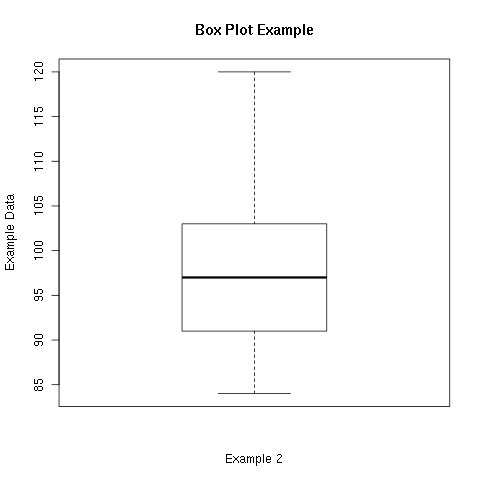
\includegraphics[width=6cm]{img/boxplotExample1}
    \end{center}

\end{frame}


\begin{frame}{Outliers}

  \begin{definition}{Outliers}

    If a number in a data set is less than Q1-$\frac{3}{2}$IQR it is
    an outlier.

    ~ \\

    If a number in a data set is more than Q3+$\frac{3}{2}$IQR it is
    an outlier.

  \end{definition}
  
\end{frame}

\begin{frame}{Example}

  \begin{tabular}{lllllllll}
    40 & 21 & 38 & 38 & 27 & 36 & 34 & 33 & 53 
  \end{tabular}

  \only<2->%
  {
    Sort the data: \\
    \begin{tabular}{lllllllll}
      21 & 27 & 33 & 34 & 36 & 38 & 38 & 40 & 53
    \end{tabular}

    Five point summary: \\
    \begin{tabular}{lllll}
      Min. & 1st Qu. & Median    & 3rd Qu. &   Max. \\
      21   & 30      & 36        & 39     & 53
    \end{tabular}
    
    The IQR is 39-30=9.

    Anything smaller than $30-\frac{3}{2}9=16.5$ is an outlier.

    Anything greater than $39+\frac{3}{2}9=52.5$ is an outlier.

  }
  
\end{frame}


\begin{frame}
  \frametitle{Z-Score}

  \begin{definition}
    Given a set of data,
    \begin{eqnarray*}
      x_1,~x_2,~x_3,\ldots,x_n,
    \end{eqnarray*}
    with sample mean $\bar{x}$ and standard deviation $s$ the
    $z$-score for a number, $x_i$, is
    \begin{eqnarray*}
      z_i & = & \frac{x_i-\bar{x}}{s}.
    \end{eqnarray*}
  \end{definition}

\end{frame}


% LocalWords:  Clarkson pausesection hideallsubsections hideothersubsections
% LocalWords:  sectionstyle IQR
